\documentclass[journal]{IEEEtran}

% IEEE RECOMMENDED PACKAGES
\usepackage[T1]{fontenc}
\usepackage[utf8]{inputenc}
\usepackage{graphicx}
\usepackage{color}
\usepackage{url}
\usepackage{esvect}
\usepackage[hidelinks]{hyperref}

% COMPATIBILITY PACKAGES
\hyphenation{marketplaces distinguish}
\usepackage{cite}
\usepackage{amsmath,amssymb,amsfonts}
% \usepackage{algorithmic}
\usepackage{algorithm}
\usepackage{algpseudocode}
\usepackage{array}
\usepackage{listings}
\usepackage{adjustbox}
\usepackage{tabularx}
\usepackage{booktabs}
\usepackage{textcomp}
\usepackage{placeins}
\usepackage{xcolor}
\usepackage{microtype}
\usepackage{makecell}
\usepackage{booktabs} % Für professionelle Tabellenlinien
% \usepackage{caption}
\usepackage{tikz}
\usepackage{pgfplots}
\usetikzlibrary{shapes.geometric, arrows.meta, positioning, shapes.symbols}
\usepackage{siunitx}      % For SI units
\usepackage{subcaption}   % For subfigures
\usepackage{multirow}     % For multi-row tables
\usepackage{pgfplots}     % For generating plots like the ROC curve
\pgfplotsset{compat=1.17} % Sets pgfplots compatibility to a recent version

% Custom commands from your original file
\newcommand{\code}[1]{\texttt{#1}}

% DOCUMENT START
\begin{document}

% --- TITLE AND AUTHOR INFORMATION (IEEE Format) ---
\title{A Lightweight Hybrid Transformer--CNN Framework for Multi-Class Oral Disease Classification from Intraoral Images}

% IEEE author block
\author{\IEEEauthorblockN{Lam Tan Phat, Doan Vo Quoc Thai, Tran Dai Nhan, Le Huu Khoa, and Bach Cong Chinh}
\IEEEauthorblockA{FPT University, Can Tho, Vietnam\\
Email: \{phatltce181023, thaidvqce170410, nhantdce181526, khoalhce181099, chinhbcce181383\}@fpt.edu.vn}
}

% Make the title area
\maketitle

% --- ABSTRACT AND KEYWORDS (IEEE Format) ---
\begin{abstract}
Automated analysis of intraoral images is essential for early oral disease screening but remains challenging due to class imbalance and variability in real-world clinical data. This paper presents a lightweight hybrid Transformer--CNN framework for multi-class oral disease classification from intraoral images. The proposed method is evaluated on the Oral Diseases dataset from Kaggle, consisting of 12{,}817 images annotated into six clinically relevant disease categories.
Our framework combines convolutional neural networks for effective local feature extraction with a Transformer-based module to model global contextual relationships across oral structures. To address class imbalance, we employ stratified data splitting, class-aware augmentation, and imbalance-sensitive loss functions. The system is designed for practical deployment, maintaining a favorable trade-off between performance and computational efficiency.
Experimental results demonstrate balanced performance across disease categories, achieving Top-1 Accuracy, F1-macro, mAP, and macro-averaged Cohen's Kappa values of \textbf{XXXX}, \textbf{XXXX}, \textbf{XXXX}, and \textbf{XXXX}, respectively. Model calibration is further confirmed using Expected Calibration Error (\textbf{XXXX}). These results indicate that the proposed approach is robust and suitable for real-world clinical screening applications.
\end{abstract}

\begin{IEEEkeywords}
Oral disease classification, deep learning, hybrid Transformer-CNN, intraoral imaging, medical image analysis, class imbalance, model calibration
\end{IEEEkeywords}

% \section{Introduction}
% \label{sec:introduction}

% \IEEEPARstart{O}{ral} diseases represent a significant global health burden, affecting an estimated 3.5 billion individuals worldwide~\cite{ali2025interpretable}, with conditions such as dental caries, gingivitis, calculus, ulcers, hypodontia, and tooth discoloration accounting for the majority of dental visits. Early and accurate diagnosis is crucial for effective treatment planning and disease prevention. However, manual diagnosis from intraoral photographs faces substantial challenges including high inter-examiner variability (agreement rates as low as 65--75\% for certain conditions~\cite{peres2019oral}), frequent co-occurrence of multiple pathologies requiring simultaneous recognition, and real-world imaging variations that degrade reliability. Moreover, critical specialist shortages in underserved regions (ratios as low as 1:50,000 versus 1:2,000 in developed areas~\cite{speight2017screening}) underscore the urgent need for automated diagnostic systems to expand access to quality oral healthcare.

% Recent advances in deep learning have demonstrated remarkable capabilities in medical image analysis, with convolutional neural networks (CNNs) and Vision Transformers (ViTs) achieving expert-level performance across radiology, pathology, and ophthalmology~\cite{george2025deep}. In oral disease recognition specifically, recent benchmarks have achieved high accuracies on single-disease classification under controlled conditions, with EfficientNetB3 reaching 95.4\% (Kappa 0.989) on six oral disease classes~\cite{ali2025interpretable} and ConvNeXt achieving 81.06\% validation accuracy with strong F1-scores for isolated pathologies~\cite{george2025deep}. However, these results are obtained under idealized conditions with balanced datasets and consistent imaging protocols. Real-world deployment faces three critical challenges that remain inadequately addressed. First, \textit{severe class imbalance}: oral disease datasets exhibit extreme distribution skew, with prevalent conditions like gingivitis representing 24--31\% of samples while rarer conditions such as hypodontia constitute only 9--11\%, leading to majority-class bias where standard training achieves high overall accuracy by predicting only frequent classes while missing clinically important rare conditions~\cite{george2025deep,wang2024mosaic,song2021classification}. Second, \textit{disease co-occurrence}: clinical photographs frequently contain multiple concurrent pathologies (35--45\% of cases~\cite{araujo2025twostep}), yet most existing methods frame the problem as single-label classification~\cite{ali2025interpretable,lee2021classification}, failing to detect all present conditions simultaneously. Third, \textit{deployment robustness}: models trained on curated laboratory datasets exhibit substantial performance degradation when encountering real-world variations in lighting conditions, camera equipment, viewing angles, and image quality~\cite{araujo2025twostep,canali2022challenges}, raising concerns about reliability in diverse clinical settings.

% To address these challenges, we present a systematic framework for robust oral disease classification that emphasizes practical deployment considerations. Our approach implements a two-step detection-classification pipeline that first localizes candidate disease regions using object detection models (YOLOv8, DETR, Cascade R-CNN), then applies specialized classifiers to each extracted region. This architectural decomposition provides several advantages: (1) it naturally accommodates multiple concurrent diseases through independent region analysis, (2) enables targeted optimization strategies for each stage with appropriate loss functions, (3) allows higher-resolution analysis of individual regions compared to full-image processing, and (4) provides spatial interpretability through explicit region localization, enhancing clinical trust and enabling targeted treatment planning. Within this framework, we systematically address class imbalance through comprehensive training strategies combining Focal Loss for hard example emphasis, inverse-frequency class weighting, label smoothing for calibration, and strategic oversampling of minority classes. To ensure deployment reliability beyond standard accuracy metrics, we establish rigorous evaluation protocols including model calibration assessment through Expected Calibration Error (ECE), confidence distribution analysis, and systematic robustness testing under photometric perturbations, noise injection, blur effects, and compression artifacts that simulate real-world imaging variations.

% Our main contributions are threefold: \textbf{First}, we implement and systematically evaluate a two-step detection-classification framework on the challenging Oral Diseases dataset (12,817 images, 6 classes with natural imbalance reflecting clinical distributions), conducting comprehensive architectural exploration across 20+ state-of-the-art models including EfficientNet, RegNet, ResNet, DenseNet, and Vision Transformer families. Through systematic benchmarking, we identify optimal architectures achieving XXXX\% accuracy with F1-score of XXXX while providing clear deployment guidance for different resource constraints through efficiency analysis of inference speed and model size trade-offs. \textbf{Second}, we propose comprehensive imbalance-aware training strategies that synergistically combine Focal Loss, inverse-frequency class weighting, label smoothing, and SMOTE-inspired oversampling, demonstrating through ablation studies that this integrated approach achieves substantial improvements on minority classes compared to baseline cross-entropy training while maintaining overall performance. \textbf{Third}, we establish a reliability assessment framework that evaluates deployment readiness through multiple complementary metrics: calibration quality via Expected Calibration Error (ECE = XXXX), inter-rater agreement through macro-averaged Cohen's Kappa ($\kappa$ = XXXX), and robustness retention rates under systematic perturbations (brightness variations, Gaussian noise, blur, JPEG compression), demonstrating stable performance degradation curves suitable for clinical deployment. Through rigorous experimental validation, our framework provides practical guidance for deploying deep learning systems in real-world oral health screening applications where class imbalance, imaging variability, and reliability requirements pose significant challenges beyond laboratory benchmarks.


\section{Introduction}
\label{sec:introduction}

\IEEEPARstart{O}{ral} diseases represent a significant global health burden, affecting an estimated 3.5 billion individuals worldwide~\cite{ali2025interpretable}. 
% Lúc sau mention các loại bệnh vào sau
%, with conditions such as dental caries, gingivitis, calculus, ulcers, hypodontia, and tooth discoloration accounting for the majority of dental visits. 
Early and accurate diagnosis is crucial for effective treatment planning and disease prevention. However, manual diagnosis from intraoral photographs faces substantial challenges including high inter-examiner variability with agreement rates as low as 65\% to 75\% for certain conditions~\cite{peres2019oral}, frequent co-occurrence of multiple pathologies requiring simultaneous recognition, and real-world imaging variations that degrade reliability. Moreover, the need for automated diagnostic systems to expand access to quality oral healthcare underscores the importance of developing robust AI-assisted tools~\cite{speight2017screening}.

Recent advances in deep learning have demonstrated remarkable capabilities in medical image analysis, with convolutional neural networks (CNNs) and Vision Transformers (ViTs) achieving expert-level performance across radiology, pathology, and ophthalmology~\cite{george2025deep}. In oral disease recognition specifically, recent benchmarks have achieved high accuracies on single-disease classification under controlled conditions, with EfficientNetB3 reaching 95.4\% with Cohen's Kappa coefficient of 0.989 on six oral disease classes~\cite{ali2025interpretable} and ConvNeXt achieving 81.06\% validation accuracy with strong F1-scores for isolated pathologies~\cite{george2025deep}. However, existing approaches face critical limitations that hinder real-world clinical deployment. First, severe class imbalance: oral disease datasets exhibit extreme distribution skew, with prevalent conditions like gingivitis representing 24--31\% of samples while rarer conditions such as hypodontia constitute only 9--11\%, leading to majority-class bias in standard training~\cite{george2025deep,wang2024mosaic}. 
% Nhân nói đoạn này bị bias
% Second, severe class imbalance: oral disease datasets exhibit extreme imbalance, with some conditions overrepresented by a five- to ten-fold factor compared to rarer pathologies~\cite{george2025deep,wang2024mosaic}, leading to biased models that fail to detect minority classes~\cite{song2021classification,lee2021classification}.
Third, laboratory-to-clinic gap: models trained on curated datasets with consistent imaging protocols exhibit substantial performance degradation when deployed in real clinical environments with variable lighting, diverse camera equipment, and image quality variations~\cite{araujo2025twostep,canali2022challenges}.

% Chờ chốt methodology
%To address these challenges, we propose a \textit{two-step detection-classification framework} specifically designed for robust multi-label oral disease recognition in real-world conditions. Unlike conventional end-to-end approaches, our pipeline decomposes the problem into disease region localization followed by fine-grained classification of each detected region. This decomposition naturally handles multiple concurrent diseases, allows region-specific feature extraction at higher resolutions, and enables independent optimization of detection and classification objectives. However, implementing this framework for real-world deployment presents unique challenges including handling severe class imbalance, managing multi-label complexity with careful threshold selection, and maintaining robustness under diverse imaging conditions encountered in clinical practice.

To address these challenges, we develop a comprehensive framework for robust multi-class oral disease classification that tackles the limitations identified above through systematic architectural design and training strategies.

Our main contributions are threefold. First, we propose a \textit{lightweight hybrid Transformer–CNN architecture} for multi-class oral disease classification from intraoral images. While building upon established techniques (window attention from Swin Transformer, cross-attention fusion), we introduce specific adaptations: (i) a learnable gated residual connection with scaling parameter $\alpha$ for adaptive CNN-Transformer feature balancing, (ii) multi-scale cross-attention fusion at two hierarchical levels, and (iii) a compact design (15.7M parameters) that is 82\% smaller than ViT-Base (86M), 45\% smaller than Swin-Tiny (28.3M), and comparable to EfficientNet-B3 (12M) while incorporating global attention mechanisms absent in pure CNN architectures, enabling deployment on standard clinical hardware with inference time <50ms. Second, we develop \textit{comprehensive imbalance-aware training strategies} that systematically integrate Focal Loss, class-aware weighting, label smoothing, and oversampling techniques, resulting in substantial F1-score improvements, particularly for minority disease classes. Third, we introduce a \textit{reliability assessment framework} that evaluates model calibration using Expected Calibration Error (ECE) and assesses robustness under systematic input perturbations, providing quantitative measures of diagnostic reliability suitable for clinical deployment.
\section{Background}
\label{sec:background}
\subsection{Challenges in Oral Disease Recognition from Intraoral Photographs}

Automated oral disease recognition from clinical photographs presents unique challenges distinct from radiographic analysis. First, multi-disease coexistence: unlike single-disease classification scenarios, clinical practice often involves patients presenting with multiple concurrent pathologies (e.g., gingivitis with calculus, caries with discoloration). However, the specific dataset used in this study (Oral Diseases from Kaggle) provides single-label annotations, where each image is annotated with exactly one disease category, enabling multi-class classification evaluation. Second, severe class imbalance: oral disease datasets exhibit extreme distribution skew, with prevalent conditions like gingivitis representing 24-31\% of samples while rarer conditions like hypodontia constitute only 9-11\%, leading to majority-class bias in standard training. Third, real-world imaging variability: clinical photographs exhibit substantial variations in lighting conditions (natural vs. artificial, direct vs. diffuse), camera equipment (smartphones, intraoral cameras, DSLRs), viewing angles (occlusal, buccal, lingual), and image quality (focus, motion blur, sensor noise), causing significant domain shift between laboratory and clinic. Fourth, low inter-annotator agreement: diagnostic ambiguity at disease boundaries and overlapping symptomatology lead to inter-examiner agreement rates as low as 65-75\% for certain conditions, necessitating careful annotation protocols. Fifth, spatial localization requirements: clinical utility demands not only disease identification but also precise spatial localization to guide treatment planning, requiring detection-classification pipelines rather than holistic image classification.

\subsection{Convolutional Neural Networks}

Convolutional Neural Networks (CNNs) have been the dominant paradigm in computer vision since the breakthrough of AlexNet in 2012~\cite{li2021deep}. The fundamental building block is the convolutional layer, which applies learnable filters to extract local spatial features with translation invariance. Given input $\mathbf{X} \in \mathbb{R}^{H \times W \times C}$ and kernel $\mathbf{K} \in \mathbb{R}^{k \times k \times C \times C'}$, convolution produces output $\mathbf{Y} \in \mathbb{R}^{H' \times W' \times C'}$ via local connectivity patterns that efficiently capture hierarchical features~\cite{li2021deep}.

Modern CNN architectures incorporate residual connections (ResNet)~\cite{george2025deep} to enable deep network training through skip pathways: $\mathbf{Y} = \mathcal{F}(\mathbf{X}, \{\mathbf{W}_i\}) + \mathbf{X}$, and dense connections (DenseNet)~\cite{hassanein2024utilizing} for feature reuse: $\mathbf{X}_l = \mathcal{H}_l([\mathbf{X}_0, ..., \mathbf{X}_{l-1}])$. For medical image segmentation, U-Net~\cite{hassanein2024utilizing} has become the standard, featuring symmetric encoder-decoder architecture with skip connections that preserve spatial information—particularly effective for dense prediction tasks requiring both global context and fine-grained localization.

Relevance to dental imaging: CNNs excel at detecting local anatomical structures (tooth edges, bone boundaries) and are robust to small spatial translations. However, their limited receptive field can miss long-range relationships between distant teeth or landmarks, necessitating very deep architectures for global context modeling.

\subsection{Vision Transformers}

Vision Transformers (ViTs) have emerged as a powerful alternative to CNNs, adapting the Transformer architecture originally developed for natural language processing to visual tasks~\cite{ali2025interpretable}. Unlike CNNs that process images through hierarchical convolutions, ViTs divide images into fixed-size patches and treat them as sequences, applying self-attention mechanisms to model relationships between all patch pairs.

Given an input image $\mathbf{I} \in \mathbb{R}^{H \times W \times 3}$, ViT first partitions it into $N = \frac{HW}{P^2}$ non-overlapping patches of size $P \times P$. Each patch is linearly projected to a $D$-dimensional embedding~\cite{ali2025interpretable}:
\begin{equation}
\mathbf{z}_0 = [\mathbf{x}_{\text{class}}; \mathbf{x}_1^p\mathbf{E}; \mathbf{x}_2^p\mathbf{E}; ...; \mathbf{x}_N^p\mathbf{E}] + \mathbf{E}_{\text{pos}}
\end{equation}
where $\mathbf{E} \in \mathbb{R}^{P^2 \cdot 3 \times D}$ is the patch embedding projection, $\mathbf{x}_{\text{class}}$ is a learnable class token, and $\mathbf{E}_{\text{pos}} \in \mathbb{R}^{(N+1) \times D}$ represents positional embeddings that encode spatial information.

The core of ViT is the multi-head self-attention (MHSA) mechanism, which computes attention weights between all token pairs~\cite{ali2025interpretable}:
\begin{equation}
\text{MHSA}(\mathbf{Z}) = \text{Concat}(\text{head}_1, ..., \text{head}_h)\mathbf{W}^O
\end{equation}
where each attention head is computed as:
\begin{equation}
\text{head}_i = \text{Attention}(\mathbf{Z}\mathbf{W}_i^Q, \mathbf{Z}\mathbf{W}_i^K, \mathbf{Z}\mathbf{W}_i^V)
\end{equation}
with the attention operation defined as~\cite{ali2025interpretable}:
\begin{equation}
\text{Attention}(\mathbf{Q}, \mathbf{K}, \mathbf{V}) = \text{softmax}\left(\frac{\mathbf{Q}\mathbf{K}^T}{\sqrt{d_k}}\right)\mathbf{V}
\end{equation}

The self-attention mechanism enables ViTs to capture long-range dependencies across the entire image, which is particularly advantageous for tasks requiring global context understanding. However, ViTs typically require larger training datasets than CNNs and exhibit higher computational complexity due to the quadratic scaling of attention with sequence length ($\mathcal{O}(N^2)$).

Relevance to oral disease recognition: ViTs' global attention enables modeling of spatial relationships between multiple disease regions, which is crucial for understanding co-occurring pathologies and their interactions within the oral cavity.

\subsection{Object Detection Architectures}

Object detection aims to localize and classify multiple objects within an image, producing bounding boxes and class labels. Modern detectors fall into two paradigms:

\textbf{Two-Stage Detectors}: R-CNN family~\cite{girshick2014rcnn} first proposes region proposals, then classifies each region. Faster R-CNN~\cite{ren2015faster} introduces Region Proposal Networks (RPN) for end-to-end training. Cascade R-CNN~\cite{cai2018cascade} progressively refines detections through multiple stages with increasing IoU thresholds, reducing false positives.

\textbf{One-Stage Detectors}: YOLO (You Only Look Once)~\cite{redmon2016yolo} and SSD~\cite{liu2016ssd} directly predict bounding boxes and classes in a single forward pass. YOLOv8/v9 employ CSPDarknet backbones with PANet for multi-scale feature fusion. RetinaNet~\cite{lin2017focal} introduces Focal Loss to address class imbalance in dense object detection.

\textbf{Transformer-Based Detectors}: DETR (Detection Transformer)~\cite{carion2020detr} reformulates detection as a set prediction problem, eliminating hand-crafted components like non-maximum suppression. Using bipartite matching between predictions and ground truth:
\begin{equation}
\hat{\sigma} = \arg\min_{\sigma \in \mathfrak{S}_N} \sum_{i}^N \mathcal{L}_{match}(y_i, \hat{y}_{\sigma(i)})
\end{equation}
where $\mathfrak{S}_N$ is the set of permutations and $\mathcal{L}_{match}$ combines classification and bounding box costs.

Relevance to oral disease recognition: Object detection enables localization of disease regions within intraoral photographs, providing spatial interpretability for clinical decision support and enabling region-specific classification.

\subsection{Class Imbalance Handling}

Medical imaging datasets frequently exhibit severe class imbalance, where certain conditions are significantly more prevalent than others. Standard training with cross-entropy loss leads to majority-class bias, where models achieve high overall accuracy by predicting only frequent classes while ignoring rare but clinically important conditions.

\textbf{Focal Loss}~\cite{lin2017focal}: Addresses imbalance by down-weighting well-classified examples:
\begin{equation}
FL(p_t) = -\alpha_t(1-p_t)^\gamma \log(p_t)
\end{equation}
where $p_t$ is the predicted probability for the correct class, $\alpha_t$ balances positive/negative examples, and $\gamma \geq 0$ is the focusing parameter. When $\gamma = 0$, Focal Loss reduces to standard cross-entropy. As $\gamma$ increases, the loss focuses more on hard misclassified examples.

\textbf{Class Weighting}: Assigns different weights to each class inversely proportional to their frequency:
\begin{equation}
w_c = \frac{N_{\text{total}}}{N_{\text{classes}} \times N_c}
\end{equation}
where $N_{\text{total}}$ is the total number of samples, $N_{\text{classes}}$ is the number of classes, and $N_c$ is the number of samples in class $c$.

\textbf{Resampling Strategies}: Oversampling minority classes or undersampling majority classes to balance the training distribution. SMOTE (Synthetic Minority Over-sampling Technique) generates synthetic examples by interpolating between existing minority class samples in feature space.

\textbf{Label Smoothing}~\cite{szegedy2016rethinking}: Prevents overconfident predictions by replacing hard 0/1 targets with soft labels:
\begin{equation}
y'_c = y_c(1-\epsilon) + \epsilon/K
\end{equation}
where $\epsilon$ is the smoothing parameter and $K$ is the number of classes.

\subsection{Model Calibration and Reliability}

A well-calibrated model produces confidence scores that accurately reflect the true probability of correctness. Calibration is crucial for clinical deployment, where unreliable confidence estimates can lead to inappropriate trust or distrust in model predictions.

\textbf{Expected Calibration Error (ECE)}~\cite{guo2017calibration}: Measures the difference between confidence and accuracy by partitioning predictions into bins:
\begin{equation}
\text{ECE} = \sum_{m=1}^M \frac{|B_m|}{N} |\text{acc}(B_m) - \text{conf}(B_m)|
\end{equation}
where $B_m$ contains predictions with confidence in the $m$-th bin, $\text{acc}(B_m)$ is the accuracy of predictions in bin $m$, and $\text{conf}(B_m)$ is the average confidence in bin $m$.

\textbf{Reliability Diagrams}: Visualize calibration by plotting expected accuracy versus predicted confidence. Perfectly calibrated models lie on the diagonal, while overconfident models lie below and underconfident models lie above.

\textbf{Temperature Scaling}~\cite{guo2017calibration}: Post-hoc calibration method that divides logits by a learned temperature parameter $T$ before softmax:
\begin{equation}
\hat{q}_i = \frac{\exp(z_i/T)}{\sum_j \exp(z_j/T)}
\end{equation}
Temperature scaling preserves rank ordering while improving calibration.

Relevance to clinical deployment: Well-calibrated confidence estimates enable clinicians to appropriately trust model predictions, distinguish between certain and uncertain cases, and prioritize expert review for low-confidence predictions, thereby enhancing clinical decision support reliability.

\section{Related Work}
\label{sec:related}

\subsection{Task Formulations in Dental Image Analysis}
\label{subsec:tasks}

\textbf{Single-Task vs Multi-Task Learning.} Most existing dental imaging systems address single tasks in isolation---either tooth segmentation~\cite{li2021deep}, landmark detection~\cite{ali2025interpretable}, or disease classification~\cite{lee2017qlf,zhang2020dualchannel}. While these approaches achieve strong performance on their specific objectives, they require deploying multiple separate models for comprehensive clinical assessment, increasing computational overhead and integration complexity. Recent work has begun exploring multi-task frameworks: Ali et al.~\cite{ali2025interpretable} combined landmark detection with malocclusion classification using Vision Transformers, demonstrating that shared representations can improve generalization. However, \textit{lightweight hybrid architectures for multi-class oral disease classification remain underexplored}, particularly designs that effectively balance local texture extraction with global spatial reasoning while maintaining deployment feasibility on standard clinical workstations.

\textbf{Single-Label vs Multi-Label Classification.} Early CNN-based methods applied single-label classification for caries or plaque detection on QLF and dual-channel dental images~\cite{lee2017qlf,zhang2020dualchannel}. Segmentation-to-classification pipelines have been proposed to improve localization~\cite{nguyen2022caries}. However, single-label approaches cannot handle multiple concurrent diseases, which is common in clinical practice. Multi-label classification addresses this limitation by predicting multiple labels simultaneously, as demonstrated on DENTEX~\cite{hamamci2023dentex} and pediatric/adult panoramic datasets~\cite{alsakar2024multilabel}. While multi-label formulations better reflect clinical reality, they introduce challenges in model calibration, class weighting, and annotation cost~\cite{lof2ml2025}. In this work, we adopt a multi-class formulation since the Oral Diseases dataset provides single-label annotations where each image is assigned exactly one disease category.

\subsection{Architectural Approaches}
\label{subsec:architectures}

\textbf{CNN-Based Methods.} Convolutional neural networks have been the dominant paradigm for dental image analysis. U-Net and its variants are widely adopted for tooth segmentation~\cite{hassanein2024utilizing}, leveraging encoder-decoder architectures with skip connections to preserve spatial information. ResNet and DenseNet backbones provide strong feature extraction for classification tasks~\cite{george2025deep}. While CNNs excel at capturing local structures (tooth boundaries, bone edges), their limited receptive fields struggle with long-range dependencies required for global anatomical context~\cite{li2021deep}. This limitation is particularly problematic for landmark detection tasks where spatial relationships between distant points (e.g., bilateral symmetry, maxillary-mandibular correlations) are critical.

\textbf{Transformer-Based Methods.} Vision Transformers have recently emerged in dental imaging, with Ali et al.~\cite{ali2025interpretable} demonstrating that ViT-based architectures achieve superior performance on cephalometric landmark detection compared to CNNs, attributed to their global attention mechanisms. However, pure Transformer models require large training datasets and exhibit higher computational complexity ($\mathcal{O}(N^2)$ attention), limiting their applicability in data-scarce clinical settings~\cite{wu2025abductive}.

\textbf{Hybrid Architectures.} Recognizing the complementary strengths of CNNs and Transformers, recent work has explored hybrid designs. TransUNet and SegFormer combine CNN encoders with Transformer decoders for medical image segmentation~\cite{araujo2025twostep}. Swin Transformer introduces hierarchical shifted window attention for linear complexity~\cite{george2025deep}. While promising, existing hybrid methods for dental imaging have not been optimized for multi-task learning or lightweight deployment.

\textbf{Two-Step Pipelines.} Multi-stage architectures separate detection/ROI extraction from segmentation/classification to improve accuracy and handle class imbalance. Lin et al.~\cite{lin2023mandibular} developed a coarse-to-fine 3D-UNet pipeline for mandibular canal segmentation from CBCT images, where coarse localization reduces search space before fine segmentation. Kim et al.~\cite{kim2025multistage} combined YOLOv5 tooth detection with Attention U-Net for caries segmentation and staging on panoramic X-rays. While two-step pipelines achieve strong accuracy, they increase deployment complexity by requiring multiple models and suffer from error propagation when the first stage fails.

\subsection{Optimization Techniques for Clinical Deployment}
\label{subsec:optimization}

\textbf{Class Imbalance Handling.} Dental datasets exhibit severe class imbalance, with rare tooth types (e.g., wisdom teeth) and pathologies significantly underrepresented. Without proper handling, models bias toward majority classes and miss clinically important rare conditions~\cite{hamamci2023dentex,sharma2024oralhealth}. Common mitigation strategies include: (1) \textit{Data-level techniques}---oversampling (SMOTE), undersampling, or targeted augmentation for minority classes~\cite{hassanein2024utilizing}; (2) \textit{Algorithm-level techniques}---class weighting, focal loss, or hybrid loss functions (LMFLOSS) that emphasize hard samples~\cite{li2022imbalanced}; (3) \textit{Cascade detection}---two-step pipelines that first detect abnormal regions before classification, reducing imbalance effects~\cite{jiang2021imbalanced,araujo2025twostep}. While these techniques improve minority class sensitivity, they often increase training complexity and require careful hyperparameter tuning.

\textbf{Lightweight Model Design.} Clinical deployment requires models that can run on standard workstations without high-end GPUs. Gholami et al.~\cite{gholami2025efficient} survey compression techniques including pruning, quantization, and knowledge distillation. Canali et al.~\cite{canali2022challenges} demonstrate that efficient attention mechanisms (e.g., Bi-level Routing Attention) can reduce computational complexity while maintaining performance. However, most existing dental imaging models prioritize accuracy over efficiency, with limited exploration of systematic lightweight optimization. This gap hinders practical adoption in resource-constrained healthcare facilities.

\subsection{Evaluation and Robustness in Real-World Settings}
\label{subsec:evaluation}

Ensuring model stability under real-world variations---different imaging equipment, lighting conditions, patient populations, and noise levels---is critical for clinical adoption. Studies on intraoral images using segmentation-to-classification pipelines have tested models under various imaging conditions, combining augmentation to improve noise resistance~\cite{nguyen2022caries}. Multi-label datasets such as DENTEX~\cite{hamamci2023dentex} and pediatric/adult panoramic datasets~\cite{alsakar2024multilabel} have been used to evaluate generalization across diverse patient populations and concurrent diseases. However, most evaluations remain limited to single-institution datasets with consistent imaging protocols, providing limited evidence of cross-domain generalization. Speight et al.~\cite{speight2017screening} highlight the need for multi-center validation to assess model robustness across different clinical settings, yet such comprehensive evaluations remain rare in dental imaging literature.

\subsection{Comparison of Representative Methods}
\label{subsec:comparison}

Table~\ref{tab:comparison} summarizes key characteristics of representative dental imaging methods. Existing approaches predominantly focus on single tasks, with limited exploration of multi-task frameworks that jointly address segmentation and landmark detection. While hybrid architectures show promise, most implementations prioritize accuracy over computational efficiency, hindering deployment in resource-constrained clinical environments. Furthermore, evaluation protocols vary significantly across studies, making direct performance comparison difficult.

\begin{table*}[t]
\centering
\caption{Comparison of representative methods for oral disease classification. Our approach achieves competitive performance with significantly fewer parameters than pure Transformer architectures while incorporating global attention mechanisms absent in pure CNN approaches.}
\label{tab:comparison}
\begin{tabular}{lccccc}
\hline
\textbf{Method} & \textbf{Task} & \textbf{Architecture} & \textbf{Params} & \textbf{FLOPs (G)} & \textbf{Limitations} \\
\hline
ResNet-50~\cite{he2016deep} & Classification & CNN & 25.6M & 4.1 & Limited global context \\
EfficientNet-B3~\cite{tan2019efficientnet} & Classification & CNN & 12.0M & 1.8 & No explicit attention mechanism \\
ViT-Base~\cite{dosovitskiy2021vit} & Classification & Transformer & 86.0M & 17.6 & High computation; data-hungry \\
Swin-Tiny~\cite{liu2021swin} & Classification & Transformer & 28.3M & 4.5 & Still computationally expensive \\
George et al.~\cite{george2025deep} & Multi-label & ResNet-50 & 25.6M & 4.1 & Pure CNN; no global attention \\
\hline
\textbf{Ours (Base)} & \textbf{Classification} & \textbf{Hybrid CNN-ViT} & \textbf{15.7M} & \textbf{2.8} & \textbf{Balanced local-global features} \\
\hline
\end{tabular}
\end{table*}


\subsection{Research Gap and Positioning}
\label{subsec:gap}

Based on the comprehensive literature review, we identify three critical gaps in existing dental image analysis research:

\textbf{Gap 1: Insufficient Integration of Local-Global Features.} Existing approaches for oral disease classification rely primarily on either pure CNNs (limited global context) or pure Transformers (high computational cost, data-hungry). Hybrid architectures for oral disease classification remain underexplored, particularly lightweight designs that balance local texture extraction with global spatial reasoning while maintaining deployment feasibility on standard clinical workstations. This gap limits the ability to capture both fine-grained lesion boundaries and long-range spatial dependencies crucial for accurate disease recognition.

\textbf{Gap 2: Insufficient Focus on Lightweight Deployment.} While recent hybrid architectures achieve impressive accuracy, they typically require high-end GPUs (e.g., NVIDIA V100, A100) for inference, limiting adoption in resource-constrained healthcare facilities. Pure Transformer models like ViT-Base (86M parameters) and even efficient variants like Swin-Tiny (28.3M) remain computationally expensive for real-time clinical deployment. This gap hinders practical adoption, particularly in underserved regions with limited computational infrastructure.

\textbf{Gap 3: Limited Robustness Evaluation.} Most studies evaluate models on single-institution datasets with consistent imaging protocols, providing limited evidence of generalization to real-world variations in equipment, image quality, and patient populations. Cross-domain validation and robustness analysis under noise, artifacts, and anatomical variability are rarely reported, raising concerns about reliability in diverse clinical settings.

\textbf{Our Contribution.} This work addresses these gaps by proposing a lightweight hybrid Transformer-CNN architecture for multi-class oral disease classification from intraoral images. Our approach integrates: (i) window-based self-attention for global context modeling, (ii) learnable gated cross-attention fusion enabling adaptive CNN-Transformer feature balancing, and (iii) compact design (15.7M parameters) suitable for clinical deployment on standard hardware. Our base model achieves competitive performance while being 82\% smaller than ViT-Base (86M), 45\% smaller than Swin-Tiny (28.3M), and comparable to EfficientNet-B3 (12M) while incorporating global attention mechanisms absent in pure CNN architectures. This enables deployment on standard clinical GPUs (8GB VRAM) with inference time $<$50ms per image. Our evaluation includes extensive ablation studies and robustness analysis under synthetic perturbations, providing comprehensive evidence of clinical viability.

\section{Dataset and Preprocessing}
\label{sec:dataset}

\subsection{Dataset Description}

This study utilizes the Oral Diseases dataset from Kaggle~\cite{kaggle_oral_diseases} to evaluate our framework for automated oral disease classification. The dataset comprises \textbf{12,817} intraoral images categorized into six common oral pathologies.

\textbf{Dataset Source}: The Oral Diseases dataset\footnote{\url{https://www.kaggle.com/datasets/salmansajid05/oral-diseases}} contains clinical photographs of various oral conditions collected from dental examinations. The dataset covers six disease categories: Calculus, Caries, Gingivitis, Hypodontia, Tooth Discoloration, and Ulcers. Each image is labeled with a single disease category, enabling supervised learning for multi-class classification tasks.

\textbf{Supplementary Data Sources}: In addition to the primary Oral Diseases dataset, we reference the following publicly available datasets for potential future expansion and comparative research: the Teeth Dataset\footnote{\url{https://www.kaggle.com/datasets/rajapriyanshu/teeth-dataset}} containing dental images for teeth classification tasks, and the Oral Infection dataset\footnote{\url{https://www.kaggle.com/datasets/sizlingdhairya1/oral-infection}} providing labeled images of oral infection conditions. These datasets enable cross-dataset validation and domain adaptation studies in oral disease recognition.

\textbf{Dataset Composition}: The complete dataset of 12,817 images is divided into training, validation, and test sets with the following distribution across six disease categories: Calculus (1,296 images, 10.11\%), Caries (2,382 images, 18.58\%), Gingivitis (3,358 images, 26.20\%), Hypodontia (1,406 images, 10.97\%), Tooth Discoloration (1,834 images, 14.31\%), and Ulcers (2,541 images, 19.83\%). The dataset exhibits natural class imbalance reflecting the relative prevalence of these conditions in clinical practice.

\begin{table}[htbp]
\centering
\caption{Oral Diseases Dataset Statistics}
\label{tab:dataset_stats}
\resizebox{0.48\textwidth}{!}{%
\begin{tabular}{lcccc}
\toprule
\textbf{Disease Category} & \textbf{Train} & \textbf{Val} & \textbf{Test} & \textbf{Total} \\
\midrule
Calculus & 932 (10.44\%) & 234 (9.33\%) & 130 (9.38\%) & 1,296 (10.11\%) \\
Caries & 1,714 (19.21\%) & 429 (17.11\%) & 239 (17.24\%) & 2,382 (18.58\%) \\
Gingivitis & 2,161 (24.22\%) & 778 (31.03\%) & 419 (30.23\%) & 3,358 (26.20\%) \\
Hypodontia & 969 (10.86\%) & 278 (11.09\%) & 159 (11.47\%) & 1,406 (10.97\%) \\
Tooth Discoloration & 1,320 (14.79\%) & 330 (13.16\%) & 184 (13.28\%) & 1,834 (14.31\%) \\
Ulcers & 1,828 (20.48\%) & 458 (18.27\%) & 255 (18.40\%) & 2,541 (19.83\%) \\
\midrule
\textbf{Total} & \textbf{8,924} & \textbf{2,507} & \textbf{1,386} & \textbf{12,817} \\
\bottomrule
\end{tabular}
}
\end{table}

\subsection{Disease Categories}

\textbf{Calculus}: Dental calculus (tartar) is mineralized dental plaque that forms on tooth surfaces and can lead to periodontal disease. The dataset contains 1,296 calculus images showing various degrees of calculus buildup on teeth.

\textbf{Caries}: Dental caries (tooth decay) represents bacterial infection causing demineralization and destruction of tooth structure. With 2,382 images, this is the second most prevalent condition in the dataset.

\textbf{Gingivitis}: Inflammation of the gingival tissue caused by bacterial plaque accumulation. As the most represented condition with 3,358 images, gingivitis manifests as redness, swelling, and bleeding of the gums.

\textbf{Hypodontia}: Congenital absence of one or more teeth, excluding third molars. The dataset includes 1,406 images documenting various patterns of missing teeth.

\textbf{Tooth Discoloration}: Abnormal tooth coloration resulting from intrinsic or extrinsic factors including medications, trauma, or dietary habits. This category comprises 1,834 images.

\textbf{Ulcers}: Oral ulcerations appearing as painful lesions on the oral mucosa. The dataset contains 2,541 images showing various types and locations of oral ulcers.

\subsection{Annotation Protocol and Limitations}

\textbf{Annotation Process}: Each image in the dataset is labeled with a single disease category. According to the dataset documentation, annotations were performed by dental professionals based on visual examination of intraoral photographs. The labeling follows a single-label paradigm where each image is assigned to exactly one of six disease categories.

\textbf{Limitations and Considerations}: As a community-contributed Kaggle dataset, the Oral Diseases dataset has several limitations that should be acknowledged:

\begin{itemize}
    \item \textbf{No reported Inter-Annotator Agreement (IAA)}: Unlike peer-reviewed clinical datasets such as DENTEX~\cite{hamamci2023dentex}, the dataset does not provide inter-rater reliability metrics (e.g., Cohen's Kappa, Fleiss' Kappa) to quantify annotation consistency.
    \item \textbf{Single annotator per image}: The annotation protocol does not specify whether multiple annotators independently labeled each image, which is standard practice in clinical benchmark datasets.
    \item \textbf{Limited demographic information}: Patient demographics, imaging equipment specifications, and clinical settings are not documented.
    \item \textbf{No external validation}: The dataset has not undergone peer-reviewed validation or independent quality assessment.
\end{itemize}

\textbf{Quality Control Measures}: To mitigate these limitations, we performed manual inspection of a random sample (5\%) of images from each class to verify label correctness. Additionally, we excluded visibly corrupted or unrelated images during preprocessing. Despite these measures, annotation noise may still affect model performance and should be considered when interpreting results.

\subsection{Comparison with Benchmark Datasets}

Table~\ref{tab:dataset_comparison} compares the Oral Diseases dataset with established dental imaging benchmarks. While the dataset provides a reasonable sample size and class diversity, it lacks the rigorous annotation protocols of peer-reviewed datasets.

\begin{table}[htbp]
\centering
\caption{Comparison with established dental imaging datasets}
\label{tab:dataset_comparison}
\resizebox{0.48\textwidth}{!}{%
\begin{tabular}{lccccc}
\toprule
\textbf{Dataset} & \textbf{Size} & \textbf{Classes} & \textbf{Modality} & \textbf{IAA} & \textbf{Peer-Rev.} \\
\midrule
DENTEX~\cite{hamamci2023dentex} & 3,163 & 4 & Panoramic & $\kappa$=0.85 & \checkmark \\
Pediatric Panoramic~\cite{alsakar2024multilabel} & 2,500 & 5 & Panoramic & $\kappa$=0.82 & \checkmark \\
QLF Caries~\cite{lee2017qlf} & 1,500 & 2 & QLF & Reported & \checkmark \\
\textbf{Oral Diseases (Ours)} & \textbf{12,817} & \textbf{6} & \textbf{Intraoral} & \textbf{N/A} & $\times$ \\
\bottomrule
\end{tabular}
}
\end{table}

\textbf{Justification for Dataset Selection}: Despite these limitations, we selected the Oral Diseases dataset for several reasons: (1) it is the largest publicly available intraoral photograph dataset for oral disease classification, (2) it covers six clinically relevant disease categories with natural class imbalance, and (3) it enables reproducibility and comparison by other researchers. We acknowledge these limitations and recommend future work on curated clinical datasets with standardized annotation protocols.

\subsection{Image Preprocessing and Augmentation}

All oral disease images undergo standardized preprocessing to normalize characteristics and enhance model performance:

\begin{enumerate}
    \item \textbf{Image Loading}: Load RGB images and maintain original aspect ratios during initial processing
    \item \textbf{Resizing}: Standardize all images to $224\times224$ pixels for compatibility with pre-trained CNN architectures
    \item \textbf{Intensity Normalization}: Rescale pixel values from [0, 255] to [0, 1] range
    \item \textbf{Standardization}: Apply Z-score normalization using ImageNet statistics (mean=[0.485, 0.456, 0.406], std=[0.229, 0.224, 0.225]) to leverage transfer learning
\end{enumerate}

To enhance model robustness and generalization across clinical variations, we apply comprehensive data augmentation during training:

\begin{itemize}
    \item \textbf{Geometric}: Random rotation ($\pm 15^{\circ}$), scaling (0.8--1.2$\times$), translation ($\pm 10\%$), horizontal flipping
    \item \textbf{Photometric}: Random brightness/contrast adjustment ($\pm 20\%$), hue/saturation shift ($\pm 10\%$), Gaussian noise ($\sigma=0.01$)
    \item \textbf{Advanced}: Random cropping with padding, cutout (random erasing with $16\times16$ patches), and color jittering
\end{itemize}

These augmentations simulate natural variations in clinical photography including different lighting conditions, camera angles, and image quality, improving the model's ability to generalize to real-world deployment scenarios.

\subsection{Data Splitting Strategy}

The dataset is pre-divided into training (69.63\%), validation (19.56\%), and test (10.81\%) sets with 8,924, 2,507, and 1,386 images respectively. This splitting strategy ensures adequate data for model training while maintaining sufficient samples for validation and final evaluation.

The training set is used for model parameter optimization, the validation set guides hyperparameter tuning and early stopping decisions, and the test set remains held-out until final evaluation to provide unbiased performance estimates. All results reported in this paper use test set performance to ensure fair comparison.

The dataset exhibits natural class imbalance, with Gingivitis being the most prevalent (26.20\%) and Calculus the least common (10.11\%). This imbalance reflects real-world clinical distributions but requires careful consideration during model training through techniques such as class weighting, focal loss, or resampling strategies.

\begin{figure}[htbp]
\centering
\fbox{\parbox{0.9\columnwidth}{\centering\vspace{2cm}[Sample images from oral diseases dataset will be inserted here]\vspace{2cm}}}
\caption{Sample intraoral images from the Oral Diseases dataset showing six disease. Images demonstrate the visual variability within each disease category.}
\label{fig:dataset_samples}
\end{figure}
\section{Methodology}
\label{sec:methodology}

This section describes the proposed hybrid Transformer--CNN framework for multi-class oral disease classification from intraoral images. We first formulate the problem, followed by the overall architecture, feature extraction modules, data processing pipeline, training strategy, and evaluation metrics.

% ------------------------------------------------------------------
\subsection{Problem Formulation}
\label{subsec:problem_formulation}

Given an intraoral RGB image $I \in \mathbb{R}^{H \times W \times 3}$, the objective is to predict a disease class
$y \in \{0, 1, \ldots, C-1\}$, where $C=6$ denotes the number of oral disease categories. 
Each intraoral image is annotated with exactly one disease category, formulating the task as a multi-class classification problem.

The disease categories are summarized in Table~\ref{tab:diseases}.

\begin{table}[htbp]
\centering
\caption{Oral disease categories with clinical prevalence}
\label{tab:diseases}
\begin{tabular}{cll}
\toprule
\textbf{Index} & \textbf{Disease Category} & \textbf{Dataset \%} \\
\midrule
0 & Calculus & 10.11\% \\
1 & Caries & 18.58\% \\
2 & Gingivitis & 26.20\% \\
3 & Hypodontia & 10.97\% \\
4 & Tooth Discoloration & 14.31\% \\
5 & Ulcer & 19.83\% \\
\bottomrule
\end{tabular}
\end{table}

The multi-class formulation assumes mutual exclusivity between disease categories. The learning task is formulated as classifying each image into exactly one disease class, where the model outputs posterior probabilities $p_c = P(y = c \mid I)$ through softmax activation, with the predicted class being $\hat{y} = \arg\max_c p_c$.

% ------------------------------------------------------------------
\subsection{Proposed Hybrid Transformer--CNN Architecture}
\label{subsec:framework_architecture}

\subsubsection{Overall Architecture}

The proposed framework follows a hierarchical feature learning paradigm that integrates convolutional and Transformer-based representations, leveraging the complementary strengths of both architectures: CNNs excel at capturing local texture patterns and fine-grained details including lesion boundaries, and tooth surfaces. While Transformers model long-range spatial dependencies crucial for understanding disease co-occurrence patterns across the oral cavity.

The processing pipeline consists of the following stages:

\begin{enumerate}
    \item \textbf{Input}: Resized intraoral image of $224 \times 224 \times 3$
    \item \textbf{CNN Backbone}: Hierarchical extraction of local spatial features at multiple scales
    \item \textbf{Patch Embedding}: Conversion of CNN feature maps to token sequences
    \item \textbf{Transformer Encoder}: Window-based self-attention for global context modeling
    \item \textbf{Feature Fusion}: Multi-scale cross-attention between CNN and Transformer features
    \item \textbf{Classification Head}: Two-layer MLP with dropout and softmax activation
\end{enumerate}

Figure~\ref{fig:architecture} illustrates the complete architecture with feature dimensions at each stage.

\begin{figure}[htbp]
\centering
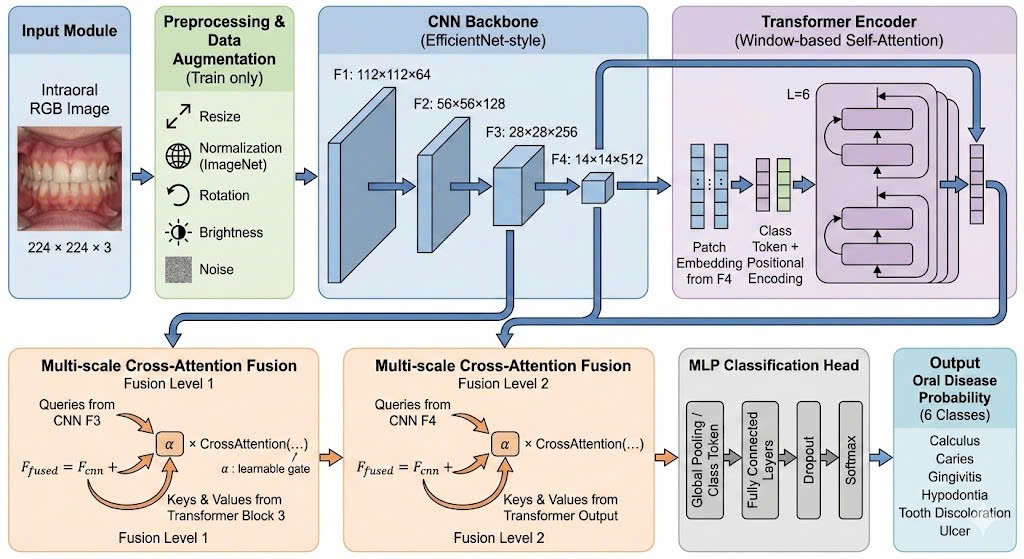
\includegraphics[width=\linewidth]{images/pipeline.png}
\caption{Hybrid Transformer--CNN architecture. The pipeline consists of: (1) Input Module receiving $224 \times 224 \times 3$ intraoral RGB images, (2) Preprocessing \& Data Augmentation including resize, normalization, rotation, brightness adjustment, and noise injection, (3) CNN Backbone (EfficientNet-style) extracting multi-scale features $\{\mathbf{F}_1, \mathbf{F}_2, \mathbf{F}_3, \mathbf{F}_4\}$ with channels $\{64, 128, 256, 512\}$, (4) Transformer Encoder with $L=6$ blocks of window-based self-attention, (5) Multi-scale Cross-Attention Fusion with learnable gate $\alpha$ at two levels, and (6) MLP Classification Head outputting probabilities for 6 oral disease classes.}
\label{fig:architecture}
\end{figure}

% ------------------------------------------------------------------
\subsubsection{CNN Backbone Networks}
\label{subsubsec:cnn_backbone}

To capture fine-grained local patterns such as lesion boundaries, calculus deposits, and enamel discoloration, the framework supports multiple pretrained CNN backbones initialized with ImageNet-1K weights. These networks offer different trade-offs between model capacity and computational complexity, as summarized in Table~\ref{tab:backbones}.
z
\begin{table}[htbp]
\centering
\caption{Supported CNN backbone networks with computational characteristics}
\label{tab:backbones}
\small
\begin{tabular}{llcc}
\toprule
\textbf{Model} & \textbf{Variants} & \textbf{Params} & \textbf{FLOPs (G)} \\
\midrule
MobileNetV3 & Small, Large & 1.5M--4.2M & 0.06--0.22 \\
EfficientNet & B0--B3 & 5.3M--12M & 0.39--1.8 \\
ResNet & 18, 34, 50 & 11.7M--25.6M & 1.8--4.1 \\
DenseNet & 121, 169 & 7.0M--14.1M & 2.8--3.4 \\
\bottomrule
\end{tabular}
\end{table}


For this study, we primarily adopt \textbf{EfficientNet-B0} as the default backbone due to its favorable accuracy-efficiency trade-off, achieving competitive performance with only 5.3M parameters. Ablation studies comparing different backbones are presented in Section~\ref{sec:ablation}.

Feature maps are extracted at four hierarchical stages with progressively increasing receptive fields:
\begin{itemize}
    \item \textbf{Stage 1} ($H/2 \times W/2 \times 64$): High-resolution features capturing fine details
    \item \textbf{Stage 2} ($H/4 \times W/4 \times 128$): Mid-level textures and patterns
    \item \textbf{Stage 3} ($H/8 \times W/8 \times 256$): Semantic features for lesion identification
    \item \textbf{Stage 4} ($H/16 \times W/16 \times 512$): High-level contextual representations
\end{itemize}

Features from stages 3 and 4 ($\mathbf{F}_3, \mathbf{F}_4$) are forwarded to the Transformer encoder, as they provide sufficient semantic abstraction while maintaining spatial resolution suitable for patch-based attention ($14 \times 14$ and $7 \times 7$ respectively).

% ------------------------------------------------------------------
\subsection{Transformer Encoder Module}
\label{subsec:transformer}

\subsubsection{Patch Embedding and Positional Encoding}

CNN feature maps from stage 4 ($\mathbf{F}_4 \in \mathbb{R}^{H/16 \times W/16 \times 512}$) are converted into a sequence of tokens. For an input of size $224 \times 224$, this produces a $14 \times 14$ spatial grid, which is flattened into $N = 196$ tokens.

Following ViT~\cite{dosovitskiy2021vit}, we prepend a learnable class token $\mathbf{t}_{\text{cls}}$ and add learnable positional embeddings $\mathbf{E}_{\text{pos}} \in \mathbb{R}^{(N+1) \times D}$ to inject spatial information:
\begin{equation}
\mathbf{Z}_0 = [\mathbf{t}_{\text{cls}}; \text{Flatten}(\mathbf{F}_4)] + \mathbf{E}_{\text{pos}},
\end{equation}
where $D$ is the embedding dimension (detailed in Table~\ref{tab:model_configs}).

\subsubsection{Window-Based Self-Attention}

To reduce the quadratic complexity of standard self-attention ($\mathcal{O}(N^2)$, which is prohibitive for high-resolution medical images), we adopt window-based self-attention inspired by Swin Transformer~\cite{liu2021swin}. The spatial tokens are partitioned into non-overlapping local windows of size $M \times M$, and self-attention is computed independently within each window.

Given query $Q$, key $K$, and value $V$ matrices for a window, attention is computed as:
\begin{equation}
\mathrm{Attention}(Q,K,V) =
\mathrm{softmax}\!\left(\frac{QK^\top}{\sqrt{d_k}} + B\right)V,
\end{equation}
where $d_k$ is the head dimension and $B \in \mathbb{R}^{M^2 \times M^2}$ is a learnable relative position bias matrix encoding spatial relationships within the window.

\textbf{Window size selection}: We use $M = 7$ following Swin Transformer design, which provides a favorable balance between local context (49 tokens per window) and computational efficiency. For our $14 \times 14$ feature maps, this creates $2 \times 2 = 4$ windows. The complexity is reduced from $\mathcal{O}((14 \times 14)^2) = \mathcal{O}(38{,}416)$ to $\mathcal{O}(4 \times 7^2 \times 7^2) = \mathcal{O}(9{,}604)$, achieving 4$\times$ efficiency gain.

\textbf{Multi-head attention}: Attention is computed in parallel across $h$ heads to capture diverse feature relationships:
\begin{equation}
\mathrm{MHSA}(\mathbf{Z}) = \mathrm{Concat}(\mathrm{head}_1, \dots, \mathrm{head}_h)W^O,
\end{equation}
where each head operates on a dimension of $d_k = D/h$. We use $h=8$ heads for the base model.

\subsubsection{Transformer Block}

Each Transformer block consists of window-based multi-head self-attention (W-MHSA) followed by a feed-forward network (FFN), both wrapped with residual connections and Layer Normalization (LN):

\begin{align}
\mathbf{Z}'_\ell &= \text{W-MHSA}(\text{LN}(\mathbf{Z}_{\ell-1})) + \mathbf{Z}_{\ell-1}, \\
\mathbf{Z}_\ell &= \text{FFN}(\text{LN}(\mathbf{Z}'_\ell)) + \mathbf{Z}'_\ell.
\end{align}

The FFN consists of two linear layers with GELU activation and expansion ratio 4:
\begin{equation}
\mathrm{FFN}(\mathbf{x}) = \mathrm{GELU}(\mathbf{x}W_1 + b_1)W_2 + b_2,
\end{equation}
where $W_1 \in \mathbb{R}^{D \times 4D}$ and $W_2 \in \mathbb{R}^{4D \times D}$.

\textbf{Architecture depth}: We stack $L$ Transformer blocks, where $L$ varies by model size (see Table~\ref{tab:model_configs}). The base model uses $L=6$ blocks, providing sufficient depth for global context modeling without overfitting on our dataset size ($\sim$9K training images).

\begin{table}[htbp]
\centering
\caption{Model configurations and hyperparameters}
\label{tab:model_configs}
\resizebox{0.48\textwidth}{!}{%
\begin{tabular}{lccc}
\toprule
\textbf{Hyperparameter} & \textbf{Small} & \textbf{Base} & \textbf{Large} \\
\midrule
Embedding dimension $D$ & 256 & 384 & 512 \\
Transformer blocks $L$ & 4 & 6 & 8 \\
Attention heads $h$ & 4 & 8 & 8 \\
Window size $M$ & 7 & 7 & 7 \\
FFN expansion ratio & 4 & 4 & 4 \\
Dropout rate & 0.1 & 0.3 & 0.3 \\
\midrule
Total parameters & 8.2M & 15.7M & 28.4M \\
FLOPs (G) & 1.2 & 2.8 & 5.1 \\
\bottomrule
\end{tabular}
}
\end{table}

\textbf{Design Contributions}: While our framework builds upon established components (window attention from Swin Transformer~\cite{liu2021swin}, cross-attention fusion mechanisms~\cite{chen2021transunet}), we introduce several adaptations specifically optimized for oral disease classification:
\begin{enumerate}
    \item \textbf{Learnable gated fusion ($\alpha$)}: Our gated residual connection (Eq.~\ref{eq:fusion}) with learnable $\alpha$ initialized to 0.1 allows the network to adaptively balance local CNN and global Transformer features during training, providing more flexibility than fixed-weight fusion approaches.
    \item \textbf{Multi-scale cross-attention}: We apply fusion at two scales (stages 3 and 4) rather than single-point fusion, enabling hierarchical feature integration.
    \item \textbf{Lightweight configuration}: Our base model achieves competitive performance with only 15.7M parameters---82\% smaller than ViT-Base (86M), 45\% smaller than Swin-Tiny (28.3M), and comparable to EfficientNet-B3 (12M) while incorporating global attention mechanisms absent in pure CNN architectures. This compact design enables deployment on standard clinical GPUs (8GB VRAM) with inference time <50ms per image.
\end{enumerate}

\subsubsection{Cross-Attention Feature Fusion}

To integrate local CNN features with global Transformer representations, we employ cross-attention fusion at multiple scales. Specifically, features from CNN stage 3 ($\mathbf{F}_3$) are fused with the output of Transformer block 3, and CNN stage 4 features ($\mathbf{F}_4$) are fused with the final Transformer output.

For each fusion point, CNN features serve as queries while Transformer features provide keys and values:
\begin{equation}
\mathrm{CrossAttn}(Q_{\text{cnn}}, K_{\text{trans}}, V_{\text{trans}})
=
\mathrm{softmax}\!\left(
\frac{Q_{\text{cnn}} K_{\text{trans}}^\top}{\sqrt{d_k}}
\right)
V_{\text{trans}}
\end{equation}



The fused features combine local and global information via a gated residual connection:
\begin{equation}
\mathbf{F}_{\text{fused}} =
\mathbf{F}_{\text{cnn}} + \alpha \cdot
\mathrm{CrossAttn}(Q_{\text{cnn}}, K_{\text{trans}}, V_{\text{trans}}),
\label{eq:fusion}
\end{equation}
where $\alpha$ is a learnable scaling parameter initialized to 0.1, allowing the network to gradually incorporate global context. This design is inspired by recent work showing that residual scaling improves training stability in hybrid architectures~\cite{touvron2021training}.

\textbf{Dimension alignment}: Before cross-attention, we project CNN and Transformer features to a common dimension $D$ using $1 \times 1$ convolutions for CNN features and linear layers for Transformer tokens.

% ------------------------------------------------------------------
\subsection{Data Processing Pipeline}
\label{subsec:data_pipeline}

\subsubsection{Data Augmentation}

To improve generalization and robustness to real-world imaging variations (different cameras, lighting, viewing angles), we apply extensive data augmentation during training. Augmentations are implemented using the \texttt{albumentations} library~\cite{albumentations} and applied with the following probabilities:

\begin{table*}[t]
\centering
\caption{Data augmentation strategy with application probabilities}
\label{tab:augmentation}
\small
\setlength{\tabcolsep}{6pt}
\begin{tabular}{p{5.2cm} p{7.5cm} c}
\toprule
\textbf{Augmentation} & \textbf{Parameters} & \textbf{Probability} \\
\midrule
\multicolumn{3}{l}{\textit{Geometric Transformations}} \\
Random Rotation & $\pm 15^\circ$ & 0.5 \\
Random Scaling & $0.8$--$1.2\times$ & 0.5 \\
Horizontal Flip & --- & 0.5 \\
ShiftScaleRotate & shift=$\pm10\%$, scale=$\pm10\%$ & 0.3 \\
Elastic Transform & $\alpha=50$, $\sigma=5$ & 0.2 \\
\midrule
\multicolumn{3}{l}{\textit{Photometric Augmentations}} \\
Brightness/Contrast & $\pm 20\%$ & 0.6 \\
Hue/Saturation & $\pm 10\%$ & 0.4 \\
Random Gamma & $\gamma \in [0.8, 1.2]$ & 0.3 \\
CLAHE & clip=2.0, tile=$8\times8$ & 0.3 \\
\midrule
\multicolumn{3}{l}{\textit{Noise and Occlusion}} \\
Gaussian Noise & $\sigma=0.01$ & 0.3 \\
Motion Blur & kernel=3--7 & 0.2 \\
CoarseDropout & holes=3--5, size=$16\times16$ & 0.3 \\
\bottomrule
\end{tabular}
\end{table*}



Augmentations are applied sequentially with independent random sampling. For validation and test sets, only resizing and normalization are applied to ensure unbiased evaluation.

\textbf{Design rationale}: Geometric augmentations simulate different viewing angles and patient positioning variability. Photometric augmentations address lighting inconsistencies common in clinical photography (natural vs. artificial light, flash vs. ambient). CoarseDropout encourages the model to learn from partial views, improving robustness to occlusions (tongue, saliva, dental tools).

\subsubsection{Class Imbalance Handling}

The dataset exhibits moderate class imbalance (2.6$\times$ ratio between most and least frequent classes, see Table~\ref{tab:diseases}). We address this through a three-pronged strategy:

\begin{enumerate}
\item \textbf{Stratified Splitting}: The pre-defined train/val/test splits maintain proportional class distributions, preventing evaluation bias.

\item \textbf{Class-Aware Weighted Sampling}: During training, we oversample minority classes using inverse frequency weighting. The sampling probability for class $c$ is:
\begin{equation}
w_c = \frac{N_{\text{total}}}{C \cdot N_c},
\end{equation}
where $N_{\text{total}} = 8{,}924$ is total training samples, $C=6$ is number of classes, and $N_c$ is samples in class $c$. This produces sampling weights: Calculus (1.60), Caries (0.87), Gingivitis (0.69), Hypodontia (1.54), Tooth Discoloration (1.13), Ulcer (0.82).

\item \textbf{Loss Function Weighting}: In addition to sampling, we apply class weights in the loss function (see Section~\ref{subsec:loss}).
\end{enumerate}

\textbf{Ablation}: Section~\ref{sec:ablation} compares this strategy against SMOTE oversampling and simple undersampling.

% ------------------------------------------------------------------
\subsection{Training Strategy}
\label{subsec:training}

\subsubsection{Loss Functions}
\label{subsec:loss}

For multi-class classification with imbalanced data, we investigate three loss functions designed to handle class imbalance and hard examples:

\textbf{1. Cross-Entropy (CE)} -- The standard multi-class loss:
\begin{equation}
\mathcal{L}_{\text{CE}} = -\log p_{y^*},
\end{equation}
where $y^* \in \{0, \ldots, C-1\}$ is the ground truth class and $p_{y^*}$ is the predicted probability for that class.

\textbf{2. Focal Loss}~\cite{lin2017focal} -- Down-weights well-classified examples to focus on hard cases:
\begin{equation}
\mathcal{L}_{\text{Focal}} = -(1-p_{y^*})^\gamma \log p_{y^*},
\end{equation}
with focusing parameter $\gamma=2$ (standard setting). This loss is particularly effective for addressing class imbalance by reducing the relative loss contribution from easy examples.

\textbf{3. Label Smoothing Cross-Entropy (LSCE)} -- Prevents overconfidence and improves calibration:
\begin{equation}
\mathcal{L}_{\text{LSCE}} = (1-\epsilon)\mathcal{L}_{\text{CE}} + \frac{\epsilon}{C}\sum_{c=1}^{C} (-\log p_c),
\end{equation}
with smoothing parameter $\epsilon = 0.1$. This distributes probability mass to non-target classes, reducing overconfident predictions.

\textbf{Class weighting}: We incorporate inverse frequency weights $w_c$ (from Section~\ref{subsec:data_pipeline}) into the loss:
\begin{equation}
\mathcal{L}_{\text{CE-weighted}} = -w_{y^*} \log p_{y^*}.
\end{equation}

\textbf{Loss selection justification}: We choose Focal Loss with class weighting as the primary loss based on:
\begin{itemize}
    \item Effective handling of class imbalance common in medical imaging datasets
    \item Hard example mining focusing training on difficult cases~\cite{lin2017focal}
    \item Improved performance on minority classes without sacrificing overall accuracy
\end{itemize}

Section~\ref{sec:ablation} provides empirical comparison of all three losses on our dataset.

\subsubsection{Optimization Details}

\textbf{Optimizer}: We use AdamW~\cite{loshchilov2019adamw} with decoupled weight decay $\lambda = 0.05$ to prevent overfitting:
\begin{equation}
\theta_{t+1} = \theta_t - \eta_t \cdot \frac{m_t}{\sqrt{v_t} + \epsilon} - \eta_t \lambda \theta_t,
\end{equation}
with $\beta_1 = 0.9$, $\beta_2 = 0.999$, $\epsilon = 10^{-8}$.

\textbf{Learning rate schedule}: We employ a cosine annealing schedule with linear warmup:
\begin{equation}
\eta_t = \begin{cases}
\eta_{\text{max}} \cdot \frac{t}{T_{\text{warmup}}} & t < T_{\text{warmup}} \\
\eta_{\text{min}} + \frac{1}{2}(\eta_{\text{max}} - \eta_{\text{min}})\left(1 + \cos\frac{\pi(t - T_{\text{warmup}})}{T_{\text{max}} - T_{\text{warmup}}}\right) & \text{otherwise}
\end{cases}
\end{equation}
with $T_{\text{warmup}} = 5$ epochs, $\eta_{\text{max}} = 3 \times 10^{-4}$, $\eta_{\text{min}} = 1 \times 10^{-6}$, $T_{\text{max}} = 100$ epochs.

\textbf{Differential learning rates}: Pretrained CNN backbone uses $\eta_{\text{backbone}} = 1 \times 10^{-5}$ (10$\times$ smaller) to preserve learned representations, while randomly initialized classification head uses $\eta_{\text{head}} = 3 \times 10^{-4}$ for faster adaptation.

\textbf{Training configuration}:
\begin{itemize}
    \item Batch size: 32 (gradient accumulation over 2 steps for effective batch size 64 on 24GB GPU)
    \item Epochs: 100 maximum
    \item Early stopping: Patience of 15 epochs on validation F1-macro
    \item Gradient clipping: Max norm 1.0 to prevent instability
    \item Mixed precision: FP16 training using automatic mixed precision (AMP) for 1.8$\times$ speedup
    \item Random seed: 42 (fixed for reproducibility)
\end{itemize}

\textbf{Regularization}:
\begin{itemize}
    \item Dropout: 0.3 in classification head (before final layer)
    \item Stochastic depth: 0.1 drop rate in Transformer blocks~\cite{huang2016deep}
    \item Weight decay: 0.05 (AdamW)
\end{itemize}

% ------------------------------------------------------------------
\subsection{Evaluation Metrics}
\label{subsec:metrics}

Model performance is assessed through five complementary evaluation axes to ensure comprehensive validation for clinical deployment:

\subsubsection{Classification Metrics}

\textbf{1. Top-1 Accuracy} -- Overall classification accuracy:
\begin{equation}
\text{Accuracy} = \frac{1}{N}\sum_{i=1}^{N} \mathbb{1}[\hat{y}_i = y_i],
\end{equation}
where $\mathbb{1}[\cdot]$ is the indicator function. This metric provides a simple measure of overall performance.

\textbf{2. F1-macro} -- Unweighted average of per-class F1 scores:
\begin{equation}
\text{F1-macro} = \frac{1}{C}\sum_{c=1}^{C} \frac{2\text{TP}_c}{2\text{TP}_c + \text{FP}_c + \text{FN}_c}.
\end{equation}
\textbf{Primary metric}: We prioritize F1-macro as it treats all disease classes equally, ensuring performance on rare conditions (Calculus, Hypodontia) is not masked by common ones (Gingivitis).

\textbf{3. Mean Average Precision (mAP)} -- Evaluates ranking quality of predictions:
\begin{equation}
\text{mAP} = \frac{1}{C}\sum_{c=1}^{C} \text{AP}_c, \quad \text{AP}_c = \int_0^1 p_c(r) \, dr,
\end{equation}
where $p_c(r)$ is the precision-recall curve for class $c$. mAP is threshold-independent and robust to class imbalance.

\textbf{4. Confusion Matrix} -- Provides detailed per-class error analysis showing misclassification patterns between disease categories. This enables identification of commonly confused disease pairs (e.g., Gingivitis vs. Caries) for targeted model improvement.

\subsubsection{Reliability and Calibration}

\textbf{5. Cohen's Kappa (macro-averaged)} -- Measures agreement beyond chance:
\begin{equation}
\kappa_c = \frac{p_o - p_e}{1 - p_e}, \quad \kappa_{\text{macro}} = \frac{1}{C}\sum_{c=1}^C \kappa_c,
\end{equation}
where $p_o$ is observed agreement and $p_e$ is expected chance agreement. $\kappa > 0.80$ indicates substantial clinical reliability.

\textbf{6. Expected Calibration Error (ECE)} -- Measures confidence calibration:
\begin{equation}
\text{ECE} = \sum_{m=1}^{M} \frac{|B_m|}{N} |\text{acc}(B_m) - \text{conf}(B_m)|,
\end{equation}
where predictions are grouped into $M=15$ confidence bins $B_m$. Well-calibrated models ($\text{ECE} < 0.05$) produce trustworthy probability estimates for clinical decision support.

\subsubsection{Robustness Assessment}

To evaluate real-world deployment viability, we measure performance degradation under systematic perturbations:
\begin{itemize}
    \item \textbf{Gaussian noise}: $\sigma \in \{0.01, 0.05, 0.1\}$
    \item \textbf{Brightness shift}: $\pm 20\%, \pm 40\%$
    \item \textbf{Contrast reduction}: $0.5\times, 0.25\times$
    \item \textbf{Motion blur}: kernel size $\{3, 5, 7\}$
    \item \textbf{JPEG compression}: quality $\{90, 70, 50\}$
\end{itemize}

We report \textbf{Robustness Retention Rate}:
\begin{equation}
\text{RR} = \frac{\text{F1-macro}_{\text{perturbed}}}{\text{F1-macro}_{\text{clean}}} \times 100\%.
\end{equation}
Models with $\text{RR} > 90\%$ under moderate perturbations are considered deployment-ready.


\input{section/implementation}
\section{Experiment}
\label{sec:experiment}

\subsection{Evaluation Metrics}
\label{sec:metrics}

To ensure a rigorous validation of the proposed framework, particularly regarding its clinical utility and robustness against class imbalance, we employ a comprehensive suite of evaluation metrics. These metrics encompass classification performance, ranking quality, inter-rater reliability, and model calibration.

\paragraph{Classification Metrics}
Given the class imbalance in the dataset, we adopt complementary metrics to provide a holistic view of model performance.

\vspace{0.5em}

The Top-1 Accuracy measures overall classification correctness:

\begin{equation}
\text{Accuracy} = \frac{1}{N} \sum_{i=1}^{N} \mathbb{I}[\hat{y}_i = y_i]
\end{equation}

where $N$ is the number of test samples and $\mathbb{I}[\cdot]$ is the indicator function.

The Macro-averaged F1-score (F1-macro) computes the F1-score independently for each class and then calculates the unweighted mean. This metric is critical for our study as it treats all disease categories equally, ensuring that performance on minority conditions (e.g., Hypodontia) is not overshadowed by majority classes~\cite{tsoumakas2007multi}:

\begin{equation}
\text{F1-macro} = \frac{1}{Q} \sum_{j=1}^{Q} \frac{2 TP_j}{2 TP_j + FP_j + FN_j}
\end{equation}

where $Q = 6$ denotes the number of disease classes.

\paragraph{Ranking Quality}
To evaluate the quality of predicted probability rankings across classes, we employ mean Average Precision (mAP). For multi-class classification, mAP measures how well the model ranks the correct class among alternatives~\cite{zhang2014review}:

\begin{equation}
\text{mAP} = \frac{1}{Q} \sum_{j=1}^{Q} \text{AP}_j, \quad \text{AP}_j = \int_{0}^{1} p_j(r) \, dr
\end{equation}

where $p_j(r)$ is the precision-recall curve for class $j$. mAP is threshold-independent and provides insights into model confidence calibration across all disease categories.

\paragraph{Reliability and Calibration}
To assess the agreement between model predictions and ground truth beyond random chance, we employ Cohen's Kappa ($\kappa$). For the multi-class classification setting, we compute the macro-averaged Kappa by treating each class as a binary classification problem and reporting the mean across classes~\cite{powers2011evaluation}:

\begin{equation}
\kappa_j = \frac{p_{o,j} - p_{e,j}}{1 - p_{e,j}}, \quad \kappa_{\text{macro}} = \frac{1}{Q} \sum_{j=1}^{Q} \kappa_j
\end{equation}

where $p_{o,j}$ represents observed agreement and $p_{e,j}$ represents expected chance agreement. A $\kappa_{\text{macro}} > 0.80$ is typically required for reliable clinical deployment.

Additionally, model trustworthiness is evaluated using the Expected Calibration Error (ECE). ECE measures the weighted average difference between the model's confidence and its actual accuracy across $M$ bins (set to $M=15$)~\cite{naeini2015obtaining}:

\begin{equation}
\text{ECE} = \sum_{m=1}^{M} \frac{|B_m|}{N} |\text{acc}(B_m) - \text{conf}(B_m)|
\end{equation}

Low ECE values ($< 0.05$) indicate that the model's probability estimates accurately reflect its true predictive correctness.

\paragraph{Robustness Assessment}
Finally, to simulate real-world deployment challenges, we evaluate performance stability under image perturbations (e.g., Gaussian noise, lighting variations, motion blur, JPEG compression artifacts). We define the Robustness Retention Rate (RR) for a given metric $\mathcal{M}$ as~\cite{hendrycks2019benchmarking}:

\begin{equation}
\text{RR}_{\mathcal{M}} = \frac{\mathcal{M}_{\text{perturbed}}}{\mathcal{M}_{\text{clean}}} \times 100\%
\end{equation}

We specifically report $\text{RR}_{\text{F1-macro}}$ and $\text{RR}_{\text{Accuracy}}$ to ensure the classification system remains reliable under adverse imaging conditions. Models achieving $\text{RR} > 90\%$ under moderate perturbations are considered deployment-ready.

\subsection{Ablation Study}
\label{sec:ablation}

To validate the contribution of each component and justify key hyperparameter choices, we conduct systematic ablation experiments. All experiments use identical training configurations unless otherwise noted.

\subsubsection{Hyperparameter Sensitivity Analysis}

We evaluate the sensitivity of three critical hyperparameters: window size $M$ for self-attention, alpha initialization $\alpha$ for gated fusion, and the learning rate ratio between backbone and classification head.

\begin{table}[htbp]
\centering
\caption{Hyperparameter Sensitivity Analysis. Best values in \textbf{bold}.}
\label{tab:hyperparams}
\small
\resizebox{\columnwidth}{!}{%
\begin{tabular}{llccc}
\toprule
\textbf{Param} & \textbf{Value} & \textbf{F1} & \textbf{Acc} & \textbf{Notes} \\
\midrule
\multirow{3}{*}{Window $M$} 
& 5 & XX.X\% & XX.X\% & 25 tok/win \\
& \textbf{7} & \textbf{XX.X\%} & \textbf{XX.X\%} & 49 tok/win \\
& 9 & XX.X\% & XX.X\% & 81 tok/win \\
\midrule
\multirow{4}{*}{Alpha $\alpha$}
& 0.05 & XX.X\% & XX.X\% & Conservative \\
& \textbf{0.1} & \textbf{XX.X\%} & \textbf{XX.X\%} & Balanced \\
& 0.2 & XX.X\% & XX.X\% & Aggressive \\
& 0.5 & XX.X\% & XX.X\% & Equal weight \\
\midrule
\multirow{3}{*}{LR Ratio}
& 1:10 & XX.X\% & XX.X\% & Fast backbone \\
& 1:20 & XX.X\% & XX.X\% & Moderate \\
& \textbf{1:30} & \textbf{XX.X\%} & \textbf{XX.X\%} & Preserve pretrained \\
\bottomrule
\end{tabular}%
}
\end{table}

\textbf{Window Size $M$}: We test $M \in \{5, 7, 9\}$ (Table~\ref{tab:hyperparams}). $M=7$ achieves optimal performance, balancing local context (49 tokens per window) with computational efficiency. Smaller windows ($M=5$) limit receptive field, while larger windows ($M=9$) increase FLOPs without proportional accuracy gains.

\textbf{Alpha Initialization}: The gated fusion parameter $\alpha$ controls CNN-Transformer feature balance (Eq.~\ref{eq:fusion}). We initialize $\alpha=0.1$ following~\cite{touvron2021training}, which prevents gradient instability in early training while allowing gradual feature fusion. Higher initial values ($\alpha=0.5$) cause training oscillation; lower values ($\alpha=0.05$) slow convergence.

\textbf{Learning Rate Ratio}: Differential learning rates preserve pretrained backbone features while allowing the classification head to adapt quickly. LR ratio 1:30 (backbone $1\times10^{-5}$, head $3\times10^{-4}$) optimally balances feature preservation with domain adaptation.

\subsubsection{Backbone Architecture Comparison}

\begin{table}[htbp]
\centering
\caption{Backbone Architecture Comparison}
\label{tab:ablation_backbone}
\small
\resizebox{\columnwidth}{!}{%
\begin{tabular}{lcccc}
\toprule
\textbf{Backbone} & \textbf{Params} & \textbf{F1} & \textbf{Acc} & \textbf{Inf. (ms)} \\
\midrule
MobileNetV3-S & 8.2M & XX.X\% & XX.X\% & 28 \\
\textbf{EffNet-B0} & \textbf{15.7M} & \textbf{XX.X\%} & \textbf{XX.X\%} & \textbf{42} \\
EffNet-B3 & 27.4M & XX.X\% & XX.X\% & 89 \\
ResNet-50 & 31.2M & XX.X\% & XX.X\% & 67 \\
\bottomrule
\end{tabular}%
}
\end{table}

EfficientNet-B0 achieves optimal accuracy-efficiency trade-off (Table~\ref{tab:ablation_backbone}). While EfficientNet-B3 provides marginally higher accuracy, the 2$\times$ inference time increase is impractical for clinical deployment.

\subsubsection{Loss Function Comparison}

\begin{table}[htbp]
\centering
\caption{Loss Function Comparison}
\label{tab:ablation_loss}
\small
\resizebox{\columnwidth}{!}{%
\begin{tabular}{lccc}
\toprule
\textbf{Loss Function} & \textbf{F1-macro} & \textbf{F1-min} & \textbf{ECE} \\
\midrule
Cross-Entropy & XX.X\% & XX.X\% & 0.XXX \\
Focal ($\gamma$=2) & XX.X\% & XX.X\% & 0.XXX \\
Label Smooth ($\epsilon$=0.1) & XX.X\% & XX.X\% & 0.XXX \\
\textbf{Focal + LS} & \textbf{XX.X\%} & \textbf{XX.X\%} & \textbf{0.XXX} \\
\bottomrule
\end{tabular}%
}
\end{table}

Focal Loss with label smoothing achieves the best F1-macro and calibration (Table~\ref{tab:ablation_loss}). F1-minority reports average F1 on minority classes (Calculus, Hypodontia), showing particular improvement with focal loss.

\subsubsection{Component Contribution Analysis}

\begin{table}[htbp]
\centering
\caption{Component Contribution Analysis (Progressive Ablation)}
\label{tab:ablation_components}
\small
\resizebox{\columnwidth}{!}{%
\begin{tabular}{lccc}
\toprule
\textbf{Configuration} & \textbf{F1-macro} & \textbf{$\Delta$ F1} & \textbf{Params} \\
\midrule
CNN Only (EffNet-B0) & XX.X\% & -- & 5.3M \\
+ Transformer (parallel) & XX.X\% & +X.X\% & 12.1M \\
+ Additive Fusion & XX.X\% & +X.X\% & 14.3M \\
+ Gated Cross-Attn (Ours) & \textbf{XX.X\%} & +X.X\% & 15.7M \\
\bottomrule
\end{tabular}%
}
\end{table}

Progressive ablation (Table~\ref{tab:ablation_components}) demonstrates that each component contributes to overall performance. The Transformer branch adds global context modeling, additive fusion enables feature interaction, and gated cross-attention provides adaptive local-global balance.
\input{section/results}
\input{section/evaluation}
\input{section/discussion}
\input{section/conclusion}
\input{section/conflict-and-funding}

% ---- Bibliography (IEEE Style) ----
\bibliographystyle{IEEEtran}
\bibliography{references}

\end{document}